\documentclass[a4paper,14pt]{extarticle} \usepackage[utf8]{inputenc}
\usepackage[T1]{fontenc}
\usepackage[margin=2.5cm]{geometry}

% Fonte Caladea se existir, senão lmodern
\IfFileExists{caladea.sty}{
  \usepackage{caladea}
}{
  \usepackage{lmodern} }
\usepackage{ragged2e}
\usepackage{graphicx}
\usepackage[portuguese]{babel}
\usepackage{wrapfig}
\usepackage{hyperref}
\usepackage{fancyhdr}
\usepackage{xcolor}
\usepackage{rotating}
\usepackage{titlesec}
\usepackage{epigraph}
\usepackage{dirtytalk}
\usepackage{indentfirst} % Indenta o primeiro parágrafo após seções

% Ajuste do recuo de parágrafo
\setlength{\parindent}{1.5em}

% Centralizar títulos
\titleformat{\section}
  {\normalfont\centering\bfseries\Large}{\thesection}{1em}{}

\titleformat{\subsection}
  {\normalfont\centering\bfseries\large}{\thesubsection}{1em}{}

\titleformat{\subsubsection}
  {\normalfont\centering\bfseries}{\thesubsubsection}{1em}{}

% -------------- Símbolos de Versículo e Resposta --------------
% Definição do símbolo (a “barrinha” inclinada)
\makeatletter
\newcommand{\vers@resp@sym}{%
  \raisebox{0.2ex}{\rotatebox[origin=c]{-20}{$\m@th\rceil$}}%
}
% macro interna que sobrepõe a barrinha e a letra V ou R
\newcommand{\vers@resp}[2]{%
  {\ooalign{%
     \hidewidth\kern#1\vers@resp@sym\hidewidth\cr
     #2\cr
  }}%
}
% comandos públicos \versicle e \response
\DeclareRobustCommand{\versicle}{\vers@resp{-0.1em}{V}}
\DeclareRobustCommand{\response}{\vers@resp{0pt}{R}}
\makeatother
% ^------------- Símbolos de Versículo e Resposta -------------^

% Rodapé com imagem e página
\pagestyle{fancy}
% ---- Cabeçalho ------------
\fancyhf[C]{}
% ----- Rodapé --------------
\fancyfoot[LO,LE]{%
  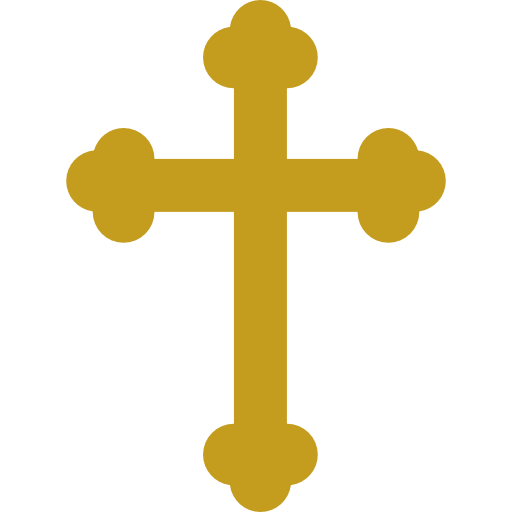
\includegraphics[scale=0.2]{assets/cross.png}\quad
  \textit{Novena a \textbf{Nossa Senhora de Schoenstatt}}
}
\fancyfoot[RO,RE]{\thepage}

\begin{document}


\begin{center}
  {\huge Novena a Nossa Senhora de Schoenstatt}
\end{center}

\say{
Uma das maiores alegrias de Maria, são os títulos que seus prediletos filhos a concedem. Incontáveis são esses ensejos dos filhos dispersos pelo mundo. Cada título quer demonstrar uma gratidão à Nossa Senhora, Mãe do Redentor.

O título atribuído a Ela, é um reconhecimento de um acontecimento, que assim poderíamos dizer, salvífico. Salvífico, porque está carregado da ação de Deus. O título expressa uma experiência religiosa de uma pessoa, ou de um grupo com o transcendente.

Neste contexto, uma experiência mariana. Atrás de cada título de Nossa Senhora tem uma linda história de fé, operado por Deus Trino, através da intercessão de Nossa Senhora. Deus Trino preferencialmente através das Causas Segundas.
}

\textbf{-- Pe. Vandemir J. Meister, ISch.}

\par\noindent\rule{\textwidth}{0.4pt}

\tableofcontents
\thispagestyle{empty}

% --- Vida / Origem da Novena ---
\newpage

\section{História}

Na Capelinha de São Miguel, no vale de Schoenstatt, em Valendar junto ao Reno, a 18 de Outubro de 1914, o Padre José Kentenich fez uma conferência à Congregação Mariana do Seminário de Schoenstatt, em que revelou uma “secreta ideia predilecta”.

A “ideia predilecta”, que ele considerou “quase demasiado ousada para o público, mas não demasiado audaz” para a pequena comunidade da Congregação, era na sua essência a seguinte: “Não seria possível que a Capelinha da nossa Congregação chegue a ser ao mesmo tempo o nosso Tabor, onde se manifeste a glória de Maria? Acção apostólica maior não poderia sem dúvida realizar, nem aos nossos vindouros, herança mais preciosa legar, do que mover Nossa Senhora e Soberana a estabelecer aqui dum modo especial o seu trono, para distribuir os seus tesouros e operar milagres de graça”.

Com estas palavras o Padre Kentenich apresentou aos jovens membros da Congregação o programa de oração e sacrifício “para fazer suave violência” à Mãe de Deus, a fim de que Ela se digne eleger a Capelinha de São Miguel como seu lugar de graças, origem e centro de um Movimento de Renovação e de Educação religioso-moral.

\subsection{Como chegou o Padre Kentenich a esta ideia?}

Nela influíram a sua fé convicta e um facto concreto. A sua fé convicta dizia que a missão e a acção da Mãe de Deus não terminaram com a sua vida terrena, mas continuam até ao fim dos tempos. Mesmo após a sua passagem para a Santíssima Trindade, Maria continua, na sua qualidade de “companheira e colaboradora permanente de Cristo em toda a Obra da Redenção”, como mais tarde o Padre Kentenich viria a designá-la, a participar activamente com toda a sua pessoa e poder de intercessão na Obra Salvífica do seu divino Filho.

Como a História da Igreja o demonstra Ela desenvolve a sua acção, de preferência, em lugares por Ela escolhidos como seus lugares de graças, e por meio de pessoas, que instrumentalmente se põem à sua disposição.

O facto concreto foi a fundação do lugar de peregrinação Valle di Pompei, em Itália, da qual o Padre Kentenich teve conhecimento pormenorizado no Verão de 1914. Se a fé e o sacrifício do advogado Bartolo Longo moveram a Mãe de Deus a fazer de Valle di Pompei um lugar da sua particular acção, não poderia suceder outro tanto em Schoenstatt, se surgissem pessoas animadas duma atitude abnegada e apostólica semelhante?

A “ideia predilecta” ateou-se nos corações dos congregados. Eles viram nela não uma ideia meramente humana, mas uma iniciativa da própria Mãe de Deus, que Maria lhes comunicou por meio do Padre Kentenich. Pela Consagração de congregados e sob a orientação do Padre Kentenich eles tomaram a iniciativa, puseram-se ao serviço da Mãe de Deus e, pela auto-educação na vida diária, entregaram-se por completo à concretização dessa “ideia predilecta”.

\subsection{Buscando uma imagem}

O Pe. José Kentenich e um grupo de rapazes, nos anos de 1914 e 1915, estavam buscando uma imagem para colocar na capelinha, local conhecido hoje como Santuário Original da Mãe Rainha.
No dia 19 de abril de 1915, foi entronizado, pelo grupos de rapazes e o Pe. Kentenich, o quadro da Mãe, Rainha Três Vezes Admirável de Schoenstatt (\textit{Mater Ter Admirábilis}- Mãe Três Vezes Admirável) no Santuário Original, na cidade de Vallendar, bairro de Schoenstatt, na Alemanha.

Este quadro foi pintado pelo artista italiano Luigi Cróssio, no século XIX. Ele também pintou um quadro, no mesmo estilo, onde São José segura o menino Jesus. O quadro da Mãe Rainha foi comprado pelo professor Huggle, que lecionava no colégio onde estudavam os rapazes que o Pe. Kentenich acompanhava espiritualmente.

Ele sabendo do desejo dos rapazes, encontrou este quadro num antiquário no sul da Alemanha, adquirindo-o. O mesmo caiu no gosto dos rapazes que estavam em busca de uma imagem mariana.

\subsection{Santuário Original}

Situado no bairro de Schoenstatt, cidade de Vallendar, foi nesse local que se originou e difundiu-se a devoção à Mãe Rainha, e posteriormente, durante a Segunda Guerra Mundial, difundiu-se a construção de Santuários idênticos a este. Por isso, o primeiro ficou nomeado de Original.

A Construção de outros Santuários idênticos surgiu da experiência da vida, experiência da vinculação ao local. Pessoas que vivenciaram uma experiência profunda de oração e espiritualidade no Santuário, queriam ter essa experiência mais perto e partilhar com outros; e assim, deu origem ao surgimento de novos Santuários da Mãe Rainha.

Hoje, para construir um Santuário da Mãe Rainha Três Vezes Admirável, pede-se autorização para a Presidência Nacional da Família da Schoenstatt, que avalia as condições, da possibilidade ou não para tal construção.

\textbf{Mãe} – Maria, primeiramente Mãe do Salvador, acompanhando todo o seu tempo de vida na região da Galileia até os últimos momentos em Jerusalém, no alto do Calvário. Ela nos foi dada como Mãe por Jesus Cristo no acontecimento da cruz: “Eis ai a tua Mãe! ” (Jo 19, 27).

Como Igreja formamos o corpo místico de Jesus Cristo tendo Maria como nossa Mãe. Inquestionável é seu papel de mãe operante na história da Igreja, e também na história pessoal de cada um dos seus filhos, principalmente aqueles que cultivam um maior vínculo de espiritualidade com Maria.

\textbf{Rainha} – Maria, em preparação à maternidade divina, foi concebida sem pecado; sendo a criatura mais perfeita, a obra-prima da criação. Na anunciação, narrado em Lucas (1,31), o Anjo disse-lhe: “Eis que conceberás e darás à luz um Filho… Ele será grande, será chamado Filho do Altíssimo, e o Senhor Deus lhe dará o trono de Davi, seu pai; ele reinará na casa de Jacó para sempre, e o seu reinado não terá fim”.

Depois de sua assunção ao céu, Ela foi coroada como Rainha do céu e da terra. Em Schoenstatt tem-se o costume de coroar Maria como Rainha, em reconhecimento por todas as obras que têm acontecido, e perscruta-se que por detrás está a mão divina.

A coroação de Maria está unida intimamente com o crescimento na Aliança de Amor que se faz com Maria. Em 10 de dezembro de 1939 foi corado Maria pela primeira vez, diante da grande dificuldade que tinha naquele então, diante no Nacional Socialismo que perseguia a Igreja e o Movimento Apostólico de Schoenstatt.

\textbf{Vencedora} – No Antigo Testamento, no relato da criação vemos o relato onde teologicamente interpleta-se o papel de Maria: “Porei inimizade entre ti e a mulher, entre tua linhagem e a linhagem dela. Ela te esmagará a cabeça…” (Gen. 3,15).

Lê-se que Deus dá os poderes para a nova mulher, que é Maria, e ela vencerá os poderes do mal. A experiência histórica das pessoas que buscavam viver a espiritualidade surgida no vale de Schoenstatt, mais especificamente o Padre José Kentenich, comprova que Maria foi a grande vencedora de todas as batalhas. Este movimento de espiritualidade por grandes perseguições passou e por todas saiu mais fortalecido, mesmo sofrendo dores.

\textbf{Três Vezes Admirável} – \textit{Mater ter Admirabilis}. A procedência desde título no remete ao padre jesuíta Jakob Rem (1546-1618) que durante uma experiência mística, solicita aos jovens que pertenciam a uma comunidade de elite da Congregação Mariana e estavam cantando as Litanias, que repetissem o título que tinham terminado de cantar, por 3 vezes.

O título era \textit{“Mater Admirábilis”} (Mãe Admirável). Esse grupo começa a usar o título Três Vezes Admirável para nossa Senhora.
O Padre Kentenich assume esse título desde o ano de 1915, atribuindo aos jovens de então, o mesmo desafio que o Pe. Jakob Rem tinha provocado nos jovens do seu tempo em Ingolstadt, sul da Alemanha, no século 17.

“A renovação da Igreja e da sociedade no seu tempo”. O Pe. Kentenich, nos seus retiros também atribui a Maria as 3 dimensões de ser Admirável: Por ser: Mãe de Deus, Mãe do Redentor e Mãe dos remidos.

\textbf{De Schoenstatt} – É um bairro na cidade de Vallendar, Alemanha, onde começou o Padre Kentenich com um grupo de jovens realizando a Aliança de Amor no dia 18 de outubro de 1914, numa capelinha, a qual conhecemos hoje como Santuário.

Antecedendo e sucedendo esse acontecimento vai-se formando a espiritualidade animada pelo Padre José Kentenich. Como ele também morava nesse local, ficou como referência a espiritualidade ali surgido.

A palavra significa “belo lugar”. Com o tempo tornou-se um local de intensas peregrinações, realizando uma “profecia” do próprio Pe. Kentenich àqueles jovens da primeira geração. Ele queria fazer daquele lugar um lugar de grandes peregrinações e que as pessoas que ali chegassem para rezar sentissem como se estivessem no Tabor: “Aqui é bom estar.”

\subsection{Formar uma Igreja}

Toda essa missão confiada por Deus através de seu instrumento Pe. José Kentenich quer perdurar através dos tempos nos seus filhos espirituais; isto é, em nós. Formar uma nova Igreja e uma nova Sociedade é um desafio para cada nova geração.

O Pe. Kentenich somente via como possibilidade essa transformação através de uma Aliança com Maria, a Aliança de Amor. Uma cultura da aliança. Temos um desafio de gerar uma nova Cultura com uma impronta mariana. Isto é, a partir de nossa Aliança de Amor com Maria queremos gestar um nobre estilo de vida que transforme a realidade.

Cultura não é aquilo que entra por nossos olhos e ouvidos, mas aquilo que transforma nossa forma de ser. Através do processo da autoeducação, formação do homem novo; queremos, talvez, ao estilo dos monges chegar ao estado de Hesychia. Hesychia é um estado de paz de espírito, mente e corpo que se alcança desde a fé; isto é, com a Graça de Deus, também dedicação humana. Gerar uma cultura do amor.

% --- Orações Diárias ---
\newpage

\section{Novena a Nossa Senhora de Schoenstatt}

\subsection{Oração Inicial} \label{oracao-inicial}
Rainha, eu creio em vosso poder. Ó Mãe Admirável, eu creio sem ver.
Vossa soberania vitoriosa me dá alento e confiança de que não falhará.

Eu vos amo, ó Mãe, que sempre me amais. Eu vos amo também quando nada me dais.
Aumentai a minha fé, a confiança e o ardor. Em tudo me dai conhecer o vosso amor.

Concede-me, ó Mãe, a graça que vos peço nesta novena \textbf{(faça o pedido)}.

\subsection{Oração Final} \label{oracao-final}

Ave Maria, por vossa pureza, conserva puro meu corpo e minha alma.

Abre-me largamente o vosso coração e o coração de vosso divino Filho. Concede-me um profundo reconhecimento de mim mesmo e a graça da perseverança até a morte. Dá-me almas e tudo mais toma-o para vós.

Vós sois três vezes admirável.
Eu sou mil vezes miserável.


Mãe, Rainha e Vencedora Três vezes Admirável, mostra-vos na minha vida.
Toma-me em vossos braços, toda vez que sou frágil.
Mostra-vos Rainha e faz do meu coração o vosso trono.
Reina em tudo o que eu fizer.
Eu vos coroo como Rainha dos meus empreendimentos, dos meus sonhos e esforços.

Mostra-vos vencedora no meu dia a dia, esmagando a cabeça da serpente do mal nas tentações que me afligem.

Vence em mim o egoísmo, a falta de fé, de esperança e de amor.

Vós sois Três vezes Admirável.
Eu sou mil vezes Miserável.
Converte-me, Mãe, para a glória de vosso Filho Jesus.
Amém.

\begin{center}
  Rezam-se 1 Pai Nosso, 3 Ave Marias, 1 Glória ao Pai.
\end{center}

\[
\textbf{Nossa Senhora de Schoenstatt, rogai por nós!}
\]

\vfill

\begin{center}
\subsection*{Fontes:}
Adaptado de: \underline{\href{https://www.maeperegrina.org.br/noticias/maria-mae-e-rainha-tres-vezes-admiravel-de-schoenstatt/}{Campanha da Mãe Peregrina de Schoenstatt}}, \underline{\href{https://www.schoenstatt.pt/sobre-schoenstatt/origem-e-historia-de-schoenstatt}{Schoenstatt}} e \underline{\href{https://formacao.cancaonova.com/espiritualidade/oracao/oracoes-a-nossa-senhora-de-schoenstatt/}{Canção Nova}}.
\end{center}


\end{document}
